\section{Real-World Experiments}

\begin{table*}[t]
\label{table:realworldSimSetups}
\centering
\begin{tabular*}{\textwidth}{lr@{\extracolsep{\fill}}rllll}
    \toprule
                                & Problem Set & Students & Q1 Size      & Q2 Size      & Q3 Size     & Q4 Size     \\
    \midrule
    Uneven Student Distribution & 293151      & 320      & 113 (35.3\%) & 100 (31.3\%) & 69 (21.6\%) & 38 (11.9\%) \\
    Even Student Distribution   & 263057      & 129      & 33 (25.6\%)  & 28  (21.7\%) & 34 (26.4\%) & 34 (26.4\%) \\
    \bottomrule
\end{tabular*}
\caption{Student totals and group distributions in the original ASSISTments data \cite{selent2016assistments} for the two problem sets of interest. Prior percent correct is discretized before removing students who have never answered incorrectly to experience the assigned condition, biasing group size towards the lower quartiles in the Uneven Student Distribution.}
\end{table*}

\begin{figure*}[t]
    \centering
    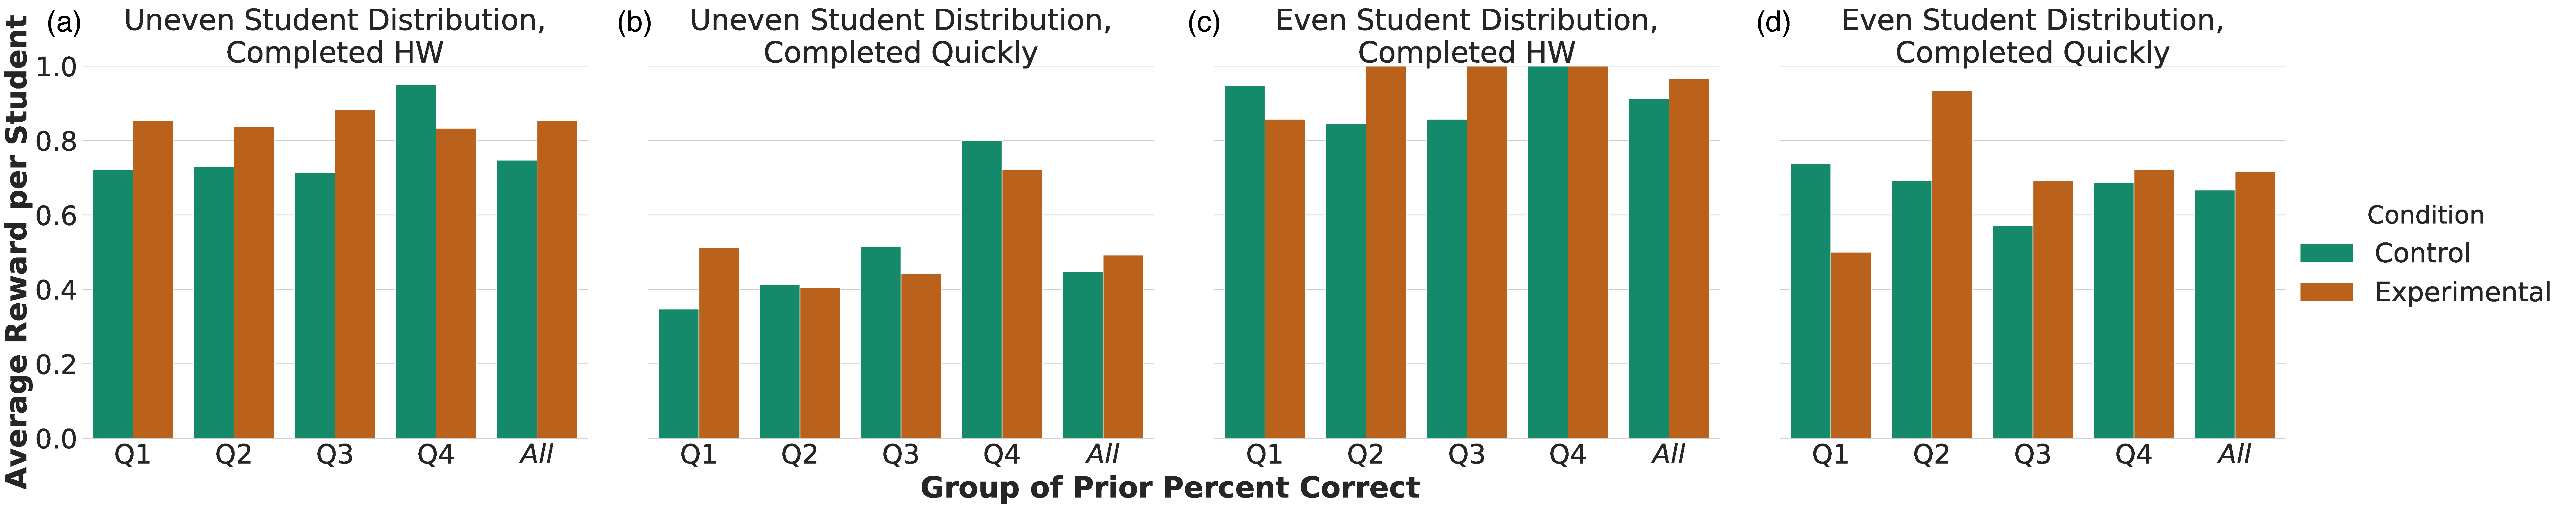
\includegraphics[width=\textwidth]{figs/RealWorld_OriginalProbsLabeled.pdf}
    \caption{Original average reward per student in the ASSISTments data \cite{selent2016assistments}, across the four quartiles (Q1--Q4) of prior percent correct and their averages, for the two conditions in the experiments (control and experimental) illustrates our model parameters of real-world scenarios.}
    %The bar graphs for the four simulation scenarios (two problem sets x two outcome measures) show average rewards across the four quartiles (Q1--Q4) and overall of prior percent correct.}
    % \caption{Average reward per student, calculated from the original ASSISTments data \cite{selent2016assistments} to show the real-world parameters, for the two conditions in the experiment (control and experimental). The bar graphs for the four simulation scenarios (two problem sets by two outcome measures) show mean reward across the four quartiles of prior percent correct (Q1--Q4) and overall.}
    \label{fig:realworldParameters}
\end{figure*}

The first two sets of simulations can guide system designers when making decisions about personalizing based on student features. However, they have some limitations: while they considered a relatively large space of possibilities for how outcomes relate to student features, they focused on showing a general variety of cases rather than on specific cases that might be most common or of particular interest in education. To address this, we conducted several case studies of how MAB algorithms would have impacted actual experiments. We consider existing experimental data in which the optimal action would be personalized to see if the contextual MAB algorithms benefits students (as would be expected from our previous simulations) and also to demonstrate how factors from the previous simulations manifest in real-world scenarios. 

The experiments were previously conducted within \textit{ASSISTments}, an online learning system, and focused primarily on middle school math. We selected several experiments from~\cite{selent2016assistments}  based on how student outcomes were related to their prior successes in the system as well as their assignment of either the control or experimental condition. Prior success in the system is a strong candidate to be a student feature for personalization: it is typically easily available and can serve as a proxy for prior knowledge, which has been shown to influence the success of different instructional strategies~\cite{shute2008focus}. 
% that we focus on were all conducted as randomized controlled trials within ASSISTments. ASSISTments is an online math learning system to teach math to students in grades 4-12 within the United States. The experiments that we focused on mainly involved middle school math students in Massachusetts. We chose several of the 22 experiments presented in previous work~\cite{selent2016assistments} based on how student outcomes were related to their prior success in the system as well as their condition assignment. Prior success in the system is a strong candidate for the type of student characteristic that designers might want to use for personalization because it can serve as a proxy for prior knowledge that is typically easily available in a system and a number of past studies have shown that prior knowledge can influence the success of different instructional strategies. 

\subsection{Methods}

To model previously collected ASSISTments data in our MAB framework, we (1) transformed both the student characteristics and the student outcomes into discrete variables,\footnote{MAB algorithms can handle non-categorical data, but we focus on the categorical case to mirror our prior simulations.} and (2) resampled from the data to generate outcomes when the MAB algorithm assigned a condition.


For step (1), we first discretized students' prior percent correct on problems within ASSISTments, the sole student feature that we included for personalization, into four quartiles: the 25\% of students who began the homework assignment with the lowest prior percent correct (Q1), then those in the 26--50\% range (Q2), and so on. The dataset contains some students who began the homework but were not assigned to a condition. Since the experiments in~\cite{selent2016assistments} mainly manipulated students' experiences (e.g. type of hint) when they answered a question incorrectly, students who have never answered incorrectly are not included in the experiment results (nor will the MAB algorithm make choices for them). However, they are included in the quartile cutoffs, which means that in the population of students with whom the MAB algorithm interacts, the number of students in each quartile may not be uniform.
% re are not necessarily an equal number of students in each quartile. Some of our simulations thus touch on the case where student characteristics are unevenly distributed.

We also chose and discretized the student outcome measures. These experiments included two different measures of student outcomes: whether each student completed the homework and the number of problems that each student answered in the homework. 
All experiments took place in the \textit{SkillBuilder} interface, where students must answer three consecutive problems correctly to complete the homework. 
Completion of homework (denoted \textit{Completed HW}) is already discrete and could easily be collected in real time; two of our simulations use this measure. 
However, it is relatively coarse, as the vast majority of students completed the homework.
% : most students do complete the homework, and they may do so even if the hints or explanations they're receiving are relatively ineffective due to external motivations. 
Thus, we also used a discretized version of the number of problems to completion (denoted \textit{Completed Quickly}). If a student completes the homework, doing so in fewer problems is a better outcome than doing so in more problems. Outcomes were based on the median problem count for students who completed the homework. Students who completed the homework in the median number of problems or fewer had positive reward, while those who did not complete the homework or completed it more slowly had no reward.
% Specifically, students who did not complete the homework were assigned no reward under this outcome measure. Then, the median of the problem count for the remaining students was used to divide their reward in a binary manner: students who completed the task in the median number of problems or below received a reward; students who took more than the median number of problems to complete did not. 
Though for practical use prior data would be needed to select an appropriate cut point, using a cut point based on collected data in our simulations measures the performance of students more closely.

% We used two types of models to evaluate MAB performance on these data, following the procedure of Rafferty, Ying and Williams (2019): parameter models and outcome models. The parameter models fit a logistic regression to the observed reward by the contextual variables of the students. Using the learned intercepts for each action and coefficients for each encoded contextual variable, the model would then run trials in the same manner as outlined in the previous methods section, using the real group proportions. Each trial in a parameter model would thus represent a classroom with similar composition and performance characteristics to the classroom from the original experiment.



% Like other recent work examining MAB behavior through simulation of experimental studies~\cite{rafferty2019statistical}, we 
% The outcome models were designed to model the classroom more directly by drawing from the observed contextual vectors and rewards. Specifically, for each of the trials, the students' context vectors were drawn in a random order, and observed rewards for each combination of action and context vectors were likewise sampled in random order. These orders remained consistent between the contextual and non-contextual MAB within a given trial, such that each trial in an outcome model would represent a classroom of students drawn with replacement from the students from the original experiment.







% \begin{figure*}[t]
%     \centering
%     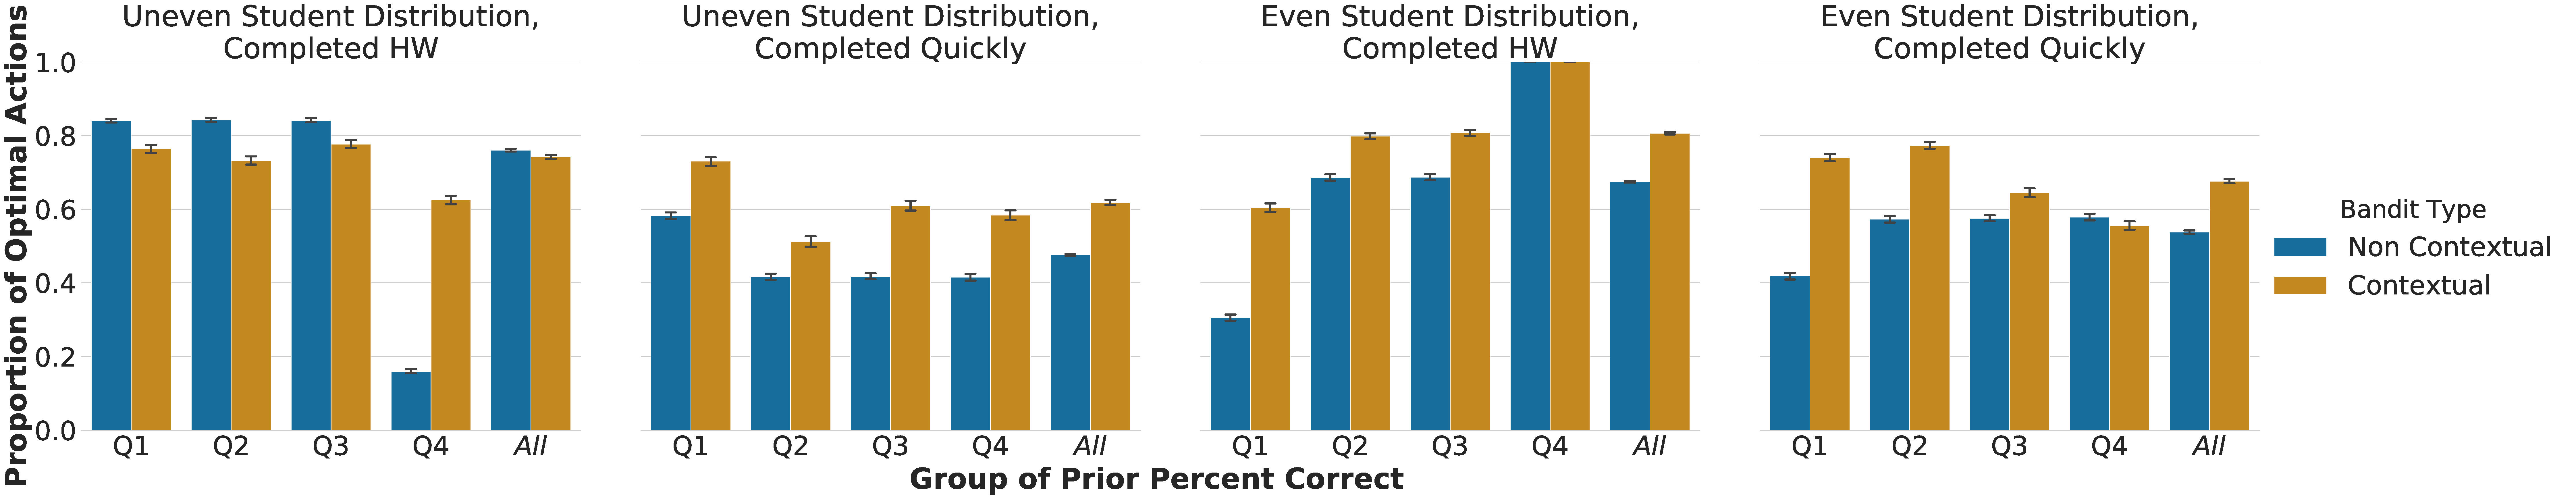
\includegraphics[width=\textwidth]{figs/RealWorld_PropOptimal.pdf}
%     \caption{Proportion of optimal actions across the four quartiles of prior percent correct (Q1--Q4) and overall for the two bandit types. 
%     %The bar graphs for the four simulation scenarios are generated by simulating classrooms with their original number of students over 1000 trials. 
%     Error bars represent 1 standard error. The extra information learned by the contextual bandit enables it to improve optimal action choice rate in most cases.}
%     \label{fig:realworldOptimal}
% \end{figure*}



% \begin{figure*}
%     \centering
%     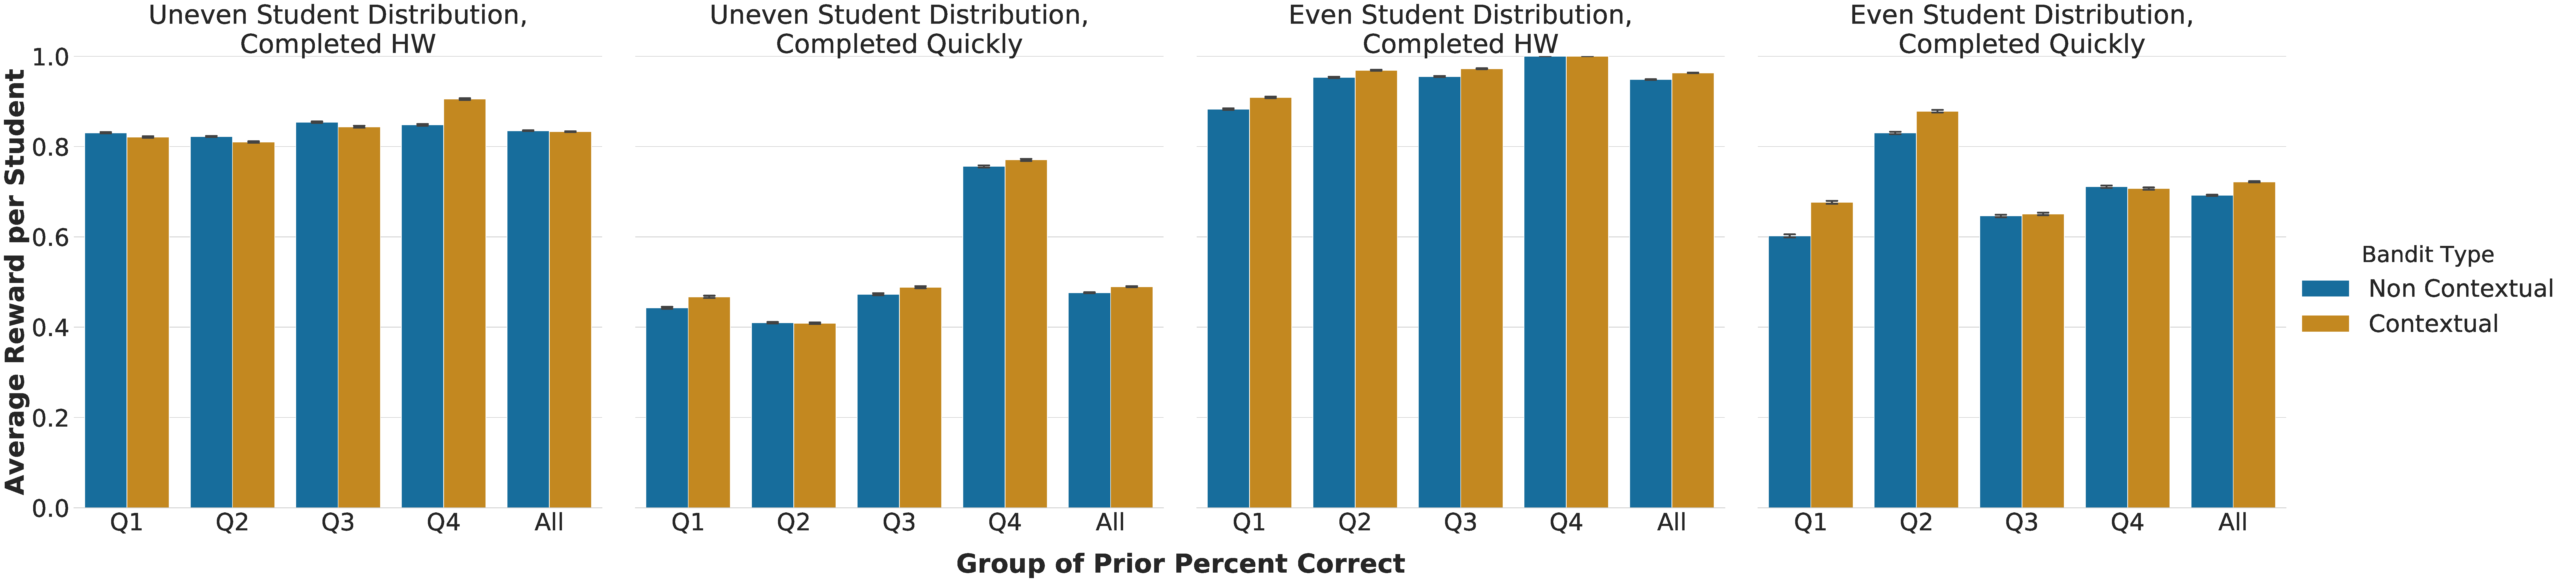
\includegraphics[width=\textwidth]{figs/RealWorld_AvgReward.pdf}
%     \caption{Average reward per student across the four quartiles of prior percent correct (Q1--Q4) and overall for the two bandit types. The bar graphs for the four simulation scenarios are generated by simulating classrooms at their original size (Table~\ref{table:realworldSimSetups}) over 1000 trials. Error bars represent 1 standard error.}
%     \label{fig:realworldReward}
% \end{figure*}

\begin{figure*}[t]
    \centering
    \includegraphics[width=\textwidth]{figs/RealWorld_SwarmHybridLabeled.pdf}
    \caption{Swarm plots for the proportion of optimal actions for the two bandit types for each quartile of prior percent correct and their averages. Each point represents results from each of the 1000 trials per experiment and the solid black lines indicate the means of each swarm plots. Points for Q4 of Even Student Distribution, Completed HW are clustered at 1.0 because both actions are optimal. The extra information learned by the contextual bandit improves performance in most cases but the bimodality for some quartiles demonstrates the associated systematic risks.}
    \label{fig:realworldDistribution}
\end{figure*}

For step (2), we simulate a MAB algorithm's performance by repeatedly sampling students from the experiment. Within each trial, we fix the number of timesteps to the total number of students in the original experiment. At each timestep, a random student is sampled, and the algorithm then selects a condition for that student.
% ; for the contextual MAB algorithm, the condition is dependent upon the student's prior percent correct.
To compute the outcome, we sample from all outcomes for students in the experiment who were in the same quartile for prior percent correct and who experienced the same chosen condition. Each trial thus represents an experiment of the same size as the original, with the students drawn with replacement from the experimental data. We randomized each of the 1000 trials, though for each trial, we use the same student ordering for both types of MAB algorithms.

In our case studies, we focus on one problem set (\#293151) where students are unevenly distributed across quartiles, with more lower-performing students (Q1), and one problem set (\#263057) in which students are more evenly distributed across quartiles (see Table~\ref{table:realworldSimSetups}).  
With the two different outcome measures, this resulted in four simulation scenarios.
We chose these problem sets because they had student outcomes that varied based on both condition and student quartile (see Figure~\ref{fig:realworldParameters}).
%, for the problem set where students were unevely distributed across quartiles, the highest performers (Q4) were helped more by the control condition than the experimental condition, while the opposite was true for the remaining students (Q1-Q3).  For the problem set with a more even distribution of students, the lowest performers (Q1) were 


\subsection{Results}

In all four settings, at least one quartile of students (out of Q1--Q4) was helped by the contextual MAB algorithm, and in three of the four settings, average outcomes across all students were improved by personalization. 


\textbf{Uneven Student Distribution, Completed HW:} As shown in Figure~\ref{fig:realworldDistribution}a, in this scenario, students in Q4 were much more likely to experience their optimal condition with a contextual MAB algorithm. This occurs because the condition that is best for the average student is the one that is worse for Q4: the non-contextual MAB thus optimizes in a way that has a systematic, negative outcome for Q4 students. Conversely, the contextual MAB algorithm does not do as well as the non-contextual algorithm for students in Q1--Q3 because of the extra exploration needed to learn about more variables that are not necessary to help these students. Overall, this means that the contextual MAB algorithm had a slightly lower rate of choosing the optimal action than the non-contextual MAB. However, the difference is relatively small, and is even smaller in terms of average reward: reward is reduced by less than $0.01$ overall, while is increased for Q4 students by about $0.06$. In this experiment, reward rates are high in general (greater than $70\%$ for all conditions and quartiles). Thus with 320 students, small differences in condition assignment often are not reflected in large differences in outcomes. Q1--Q3 students have very similar outcomes across the two methods of condition assignment; Q4 has the greatest difference in success for one condition versus another, and thus the large increase in optimal condition assignment for these students does boost the average outcomes. 

\textbf{Uneven Student Distribution, Completed Quickly:} Using the Completed Quickly outcome measure with the same students, students in all quartiles were more likely to be assigned to the optimal condition when the contextual MAB algorithm was used (Figure~\ref{fig:realworldDistribution}b). This pattern occurs because the overall probability of a positive outcome is very similar across the two conditions when student quartiles are ignored (shown by \textit{All} in Figure~\ref{fig:realworldParameters}b), making it difficult for the non-contextual bandit to learn that the experimental condition is better on average. In contrast, the differences between conditions are large for all quartiles except Q2. Thus, the information from the student quartiles makes the problem easier for the contextual MAB algorithm, though the relatively small difference between conditions for Q2 results in the lowest overall proportion of optimal action choices. This simulation thus importantly shows a scenario that was not explored in the prior simulations, in which knowing about extra information increases the number of  parameters to learn but makes learning about each of those individual parameters easier.

\textbf{Even Student Distribution, Completed HW:} For this scenario, there were again very high reward probabilities across all conditions, and a relatively small overall difference between conditions but larger differences between conditions for three of the four quartiles. The results from the previous simulation were mirrored here: all groups with some reward rates of less than $100\%$ were aided by the contextual MAB algorithm.

\textbf{Even Student Distribution, Completed Quickly:} Finally, using the Completed Quickly outcome measure for this second set of students, the results were still largely in favor of the contextual MAB algorithm. As the experimental condition is better on average, students in Q1 experience a large positive impact through personalization because the control condition is uniquely better for them. Q2 and Q3 also experience positive impacts, with the impact on Q2 students being larger because the difference between the two conditions is larger, which speeds learning for the contextual bandit. Conversely, Q4 students experience slightly less positive outcomes under the contextual MAB algorithm because the small difference between conditions slows learning; in comparison, the contextual MAB algorithm is more beneficial for Q4 students since the overall difference between conditions across all students is larger than the difference for Q4 students only. 

% in comparison, the overall difference across all students is larger between conditions than the difference only for Q4 students, so the non-contextual MAB algorithm uses this information and is thus more beneficial for Q4 students than the contextual MAB algorithm.

\textbf{Variability in real-world scenarios:} Variability across trials in these scenarios showed the same trend as in the previous simulations: the non-contextual MAB algorithm typically has slightly more variation around the mean of the distribution, but only the contextual MAB algorithm shows bimodality, with some trials showing very poor performance for at least one of the groups (Figure~\ref{fig:realworldDistribution}). 




















\begin{comment} We first modeled problem set 293151 with a completion reward scheme, under which students from quartiles 1--3 of Prior Percent Correct performed better under condition E, while students from quartile 4 performed better under condition C (see Table~\ref{table:observedParamsP293151}). As this was an example of group-dependent policy, we hypothesized that students from quartile 4, as the minority, would receive considerably more reward from the use of a contextual MAB compared to a non-contextual MAB, while the other groups would see slightly diminished reward, similar to the group dependent policy simulation shown above.

\begin{table}[h]
\label{table:observedParamsP293151}
\centering
\begin{tabular}{cc||c|c|c|c}
                           &   & \multicolumn{4}{c}{Accuracy Quartile}      \\
                           &   & $Q_1$  & $Q_2$  & $Q_3$  & $Q_4$  \\\hline\hline
\multirow{2}{*}{Condition} & C & 0.72   & 0.73   & 0.71   & 0.95   \\\cline{2-6}
                           & E & 0.83   & 0.83   & 0.87   & 0.77    
\end{tabular}
\caption{Observed student probability of completion for problem set 293151.}
\end{table}

As shown in the Table~\ref{table:observedParamsP293151}, for 375 students, quartiles 1--3 did indeed see slightly diminished reward (-1.020243 for quartile 0; -1.037975 for 1; -0.292887 for 2); however, the gain in reward for quartile 3 was also considerably slight (+2.866426). While these results are not in direct conflict with those from the group dependent policy simulation shown above, the end result is that total classroom reward for this problem set was considerably lower with a contextual MAB than with a non-contextual MAB, despite the group dependent policy. We believe that this is because the minority group is quartile 4 and has high reward and low variance. Therefore, the contextual bandit is less likely to explore and optimize effectively for that minority group. We hypothesized that if the minority group is quartile 1 and has low reward, then the contextual bandit should be able to explore and optimize effectively. 

In order to test this hypothesis, we next modeled problem set 263057 with the same completion reward scheme, under which students from quartile 1 performed better under condition C while students from quartiles 2--3 performed better under condition E, with similarly high proportions of reward in all quartiles as seen in problem set 293151 (see Table~\ref{table:observedParamsP263057}). Students from quartile 4 performed equally under both conditions, and thus this set was not a perfect match for our archetype for group-dependent policy, and that, assuming the null hypothesis, we would expect to see less gain in reward for quartile 1 in this case than for quartile 4 for the prior.

\begin{table}[h]
\label{table:observedParamsP263057}
\centering
\begin{tabular}{cc||c|c|c|c}
                           &   & \multicolumn{4}{c}{Accuracy Quartile}      \\
                           &   & $Q_1$  & $Q_2$  & $Q_3$  & $Q_4$  \\\hline\hline
\multirow{2}{*}{Condition} & C & 0.95   & 0.85   & 0.86   & 1.00 \\
                           & E & 0.86   & 1.00   & 1.00   & 1.00    
\end{tabular}
\caption{Observed student probability of completion for problem set 263057.}
\end{table}

Table~\ref{table:observedParamsP263057} shows the results: as expected, for 129 students, we found that the contextual MAB received slightly diminished reward relative to the non-contextual MAB for quartiles 2--4 ({-#} for quartile 2; {-#} for 3; {-#} for 4), but considerably increased reward for quartile 1 ({+#}). These results indicate that high probabilities influence the effectiveness of MAB models due to two factors: first, less reward is available to gain relative to the least beneficial condition; second, lower variance increases the likelihood that the MAB (especially contextual) will exploit the non-optimal condition. {...}

Next, we moved to modeling with observed difficulty reward in order to more closely match the probabilities of reward we had assumed in the simulations. We again worked with problem set 263057 which, under this reward scheme, saw students from quartile 1 performing better under condition C and students from quartiles 2--4 performing better under condition E, each by a substantial margin (see Table below). We hypothesized, as with the first experiment, that we would see performance differences similar to those observed in those in the simulation section above

\begin{table}[]
\begin{tabular}{lllll}
  & 0    & 1    & 2    & 3    \\
C & 0.74 & 0.69 & 0.57 & 0.69 \\
E & 0.50 & 0.93 & 0.69 &0.72    
\end{tabular}
\end{table}

However, this experiment also exhibited behavior that we had not considered in the simulations: as shown in Table {Y}, not only did the minority group, quartile 1, see great gain with the contextual MAB over the non-contextual (+1.425619), but the majority, quartiles 2--4, also benefited considerably (+0.795122 for quartile 1; +0.039711 for 2; +0.050724 for 3). {...}

Lastly, we modeled problem set 241622 with an observed difficulty reward scheme. These parameters saw students from all quartiles performing better under condition {C/E}, though by differing margins (see Table {X}), thus following a group-independent policy, group dependent reward pattern. As such, we hypothesized that our earlier finding from {Simulation X.Z} should hold that whenever the policy is group-independent, regardless of whether a contextual model would be more accurate to the data, the non-contextual MAB will produce better rewards.

The results, shown in Table {Y}, indicate that this principle holds in a modeled experiment: all groups saw diminished reward from the contextual MAB relative to the non-contextual MAB. Consistent with our findings in {Simulation X.Z}, while  
\end{comment}






